
\documentclass[crop, tikz, border=0pt]{standalone}
\usetikzlibrary{matrix}
\usetikzlibrary{patterns}
\usepackage{varwidth}
\usepackage{amsmath}
\usepackage{amssymb}
\usepackage{color}
\begin{document}
\color{white}
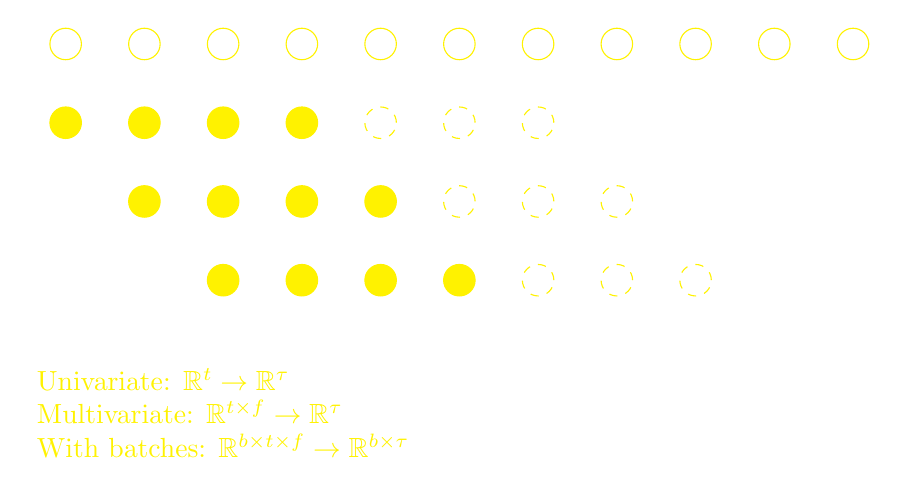
\begin{tikzpicture}[draw=yellow]
%\tikzset{rectangle node/.style = {rectangle, inner sep=1pt, draw, fill=white}}
\tikzset{edge/.style = {->,> = latex, line width=.5 pt}}

   
\foreach \x in {0, 1, 2, 3, 4, 5, 6, 7, 8, 9, 10}
   {\draw (\x, 0) circle (.2);}

\foreach \x in {0, 1, 2, 3}
  {\draw [fill=yellow] (\x, -1) circle (.2);}

\foreach \x in {4, 5, 6}
{\draw [dashed] (\x, -1) circle (.2);}

\foreach \x in {1, 2, 3, 4}
{\draw [fill=yellow] (\x, -2) circle (.2);}

\foreach \x in {5, 6, 7}
{\draw [dashed] (\x, -2) circle (.2);}

\foreach \x in {2, 3, 4, 5}
{\draw [fill=yellow] (\x, -3) circle (.2);}

\foreach \x in {6, 7, 8}
{\draw [dashed] (\x, -3) circle (.2);}   



 \node[below, color=yellow, align=left] at (2, -4) {
 Univariate: $\mathbb  R^{t} \rightarrow \mathbb{R}^{\tau}$ \\
 Multivariate: $\mathbb  R^{t\times f} \rightarrow \mathbb R^{\tau}$ \\
 With batches: $\mathbb  R^{b \times t\times f} \rightarrow \mathbb R^{b\times\tau}$
}; 
    
\end{tikzpicture}
\end{document}